%%January 20- 2002
%\documentclass[wrr]{agu2001}
\documentclass{report}


\usepackage{natbibDK}
\usepackage{amsmath}
\usepackage{amssymb}
\usepackage[dvips]{graphicx}


\usepackage[T1]{fontenc}        %for danish letters
\usepackage[latin1]{inputenc}   %for danish letters




\begin{document}

%% ------------------------------------------------------------------------ %%
%
%  TITLE
%
%% ------------------------------------------------------------------------ %%


\title{Formler til Milj\ostyrrelsen}

%% ------------------------------------------------------------------------ %%
%
%  AUTHORS AND AFFILIATIONS
%
%% ------------------------------------------------------------------------ %%

\author{Mikkel Mollerup}




\chapter{Water movement}


\section{Richard's Equation}

The water flow in porous media can be described with the formula
of Richard. The equation is here derived. The water flux density
vector, $\mathbf{q}$ can be calculated by the Darcy�s law. For a
two-dimensional vertical transect it yields:
\begin{equation}
\mathbf{q}=-\mathbf{K}(\psi)\nabla(\psi + z) \label{eq:darcy}
\end{equation}
where $\mathbf{K}(\psi)$ is the hydraulic conductivity tensor,
$\psi$ is the potential head. The x-axis is chosen in horizontal
direction and the z-axis is positive upwards. The conductivity
tensor can be expressed as:
\begin{equation}
\mathbf{K}=\begin{bmatrix} K_{xx} & K_{xz} \\ K_{zx} & K_{zz}
 \end{bmatrix}
\end{equation}
For the model with rectangular cells we have chosen that the
 principal directions of the anisotropic medium are parallel with
 the $x$- and $z$-axis, i.e.
\begin{equation}
\mathbf{K}=\begin{bmatrix} K_{xx} & 0 \\ 0 & K_{zz}
 \end{bmatrix}
\end{equation}
The mass balance for the system gives
\begin{equation}
\frac{\partial \theta}{\partial t}=-\nabla \cdot \mathbf{q}
-\Gamma \label{eq:continuity}
\end{equation}
where $\theta$ is the water content and $\Gamma$ is the sink term.
The partial differential equation can be developed by combining
Darcy�s law, equation \ref{eq:darcy} and the mass balance,
equation \ref{eq:continuity}, thus
\begin{equation}
\frac{\partial \theta}{\partial t}=\nabla \cdot
\left(\mathbf{K}(\psi)\nabla (\psi + z)\right) - \Gamma
\label{eq:richards}
\end{equation}
This is known as Richard's equation. For the modeling is assumed
that the soil-water retention is without hysteresis, i.e. there is a
unique relation between the matric pressure potential and the water
content.

To solve Richard's equation it is necessary to specify initial and
boundary conditions. The boundary conditions specify a combination
of $\psi$ and its derivative on the boundary. In the prototype it
is possible to use different forms of flux (Neumann) and
predescribed pressure (Dirichlet) boundary conditions. The problem
to be solved for determining the water movement can be summarized
to
\begin{equation}
\begin{cases}
\frac{\partial \theta}{\partial t}=\nabla \cdot
\left(\mathbf{K}(\psi)\nabla (\psi + z) \right)-\Gamma & \text{in}\  \Omega \\
\mathbf{\bar{n}} \cdot \left(\mathbf{K}(\psi)\nabla (\psi + z)
\right)=
-q & \text{on}\ \partial \Omega^{N} \\
\psi=\psi_0 & \text{on}\ \partial \Omega^{D}
\end{cases}
\label{eq:watermovement}
\end{equation}
where $\mathbf{\bar{n}}$ is the outward unit normal, and $q$ is the
size of the size of the outward flow from the domain. $\psi_0$ is
the predescribed pressure at the boundary. $\partial\Omega^{N}$ and
$\partial\Omega^{D}$ are part of the boundary with Neumann and
Dirichlet boundaries, respectively such that
$\partial\Omega=\partial\Omega^{N} \cup \partial\Omega^{D}$. Each of
$\partial\Omega^{N}$ and $\partial\Omega^{D}$ are not necessarily
one continuous curve piece. For lower boundary condition is a
special case of the Neumann boundary conditions often applied. It
here assumed that the flow it is only driven by the gravity (gravity
boundary condition), i.e. $\partial \psi/
\partial x= \partial \psi/ \partial z=0$ which gives
\begin{equation}
q=\mathbf{\bar{n}} \cdot \begin{bmatrix}0 \\ K_{zz}
\end{bmatrix}
\end{equation}
Another often used boundary condition is the seepage boundary
  condition where we for $\psi>0$ have specified pressure
  corresponding to the depth of the overlaying water. For $\psi \leq0$
  have specified flow to be equal to 0, i.e. a Dirichlet boundary
  condition for $\psi>0$ and a Neumann boundary condition for $\psi
  \leq 0$.





\section{Finite Volume Method}


\subsection{Mesh}


In Daisy2D, the domain, $\Omega$ is divided into $N$ non-overlapping
polygons, also denoted control volumes or cells. In Daisy2D it
should be possible to choose between grids consisting of only
rectangular cells or meshes consisting of trapezoids with two
vertical faces. Figure \ref{fig:grid_rect} shows a grid only
consisting of rectangular cells. The domain $\Omega$ in the figure
is in divided into 3 subdomains, each consisting of a whole number
of cells. Each subdomain can contain different soils with different
hydraulic properties. The grid shown in figure \ref{fig:grid_trapz}
consists of trapezoids (where most of them also are rectangles).
Only in the proximity of the drainpipe (see figure
\ref{fig:grid_trapz_part}), the cells are not rectangular.


\begin{figure}[h]
\includegraphics[width=\hsize]{grid_rect.eps}
\caption{Example of grid consisting of rectangular cells.}
\label{fig:grid_rect}
\end{figure}

\begin{figure}[h]
\includegraphics[width=\hsize]{grid_trapz.eps}
\caption{Example of grid consisting of trapezoids.}
\label{fig:grid_trapz}
\end{figure}

\begin{figure}[h]
\includegraphics[width=\hsize]{grid_trapz_part.eps}
\caption{Close picture of grid near the drain pipe.}
\label{fig:grid_trapz_part}
\end{figure}


The quadrilateral (rectangular or trapezoid) cells are denoted $Q_i$
where $i=1,2,\cdots, N$. $|Q_i|$ denotes the area of $Q_i$, and
$\partial Q_i$ is the boundary of $Q_i$ i.e. the edges (or faces) of
$Q_i$. All internal edges $e_{ij}$ are labeled by indices, $i$ and
$j$ of the adjacent cells that shares face. The grid is constructed
such that only whole faces are shared ($e_{ij}=Q_i \cap Q_j$). The
length of $e_{ij}$ is $|e_{ij}|$ and the unit normal vector pointing
from $Q_i $into $Q_j$ and orthogonal to $e_{ij}$ is denoted
$\bar{\mathbf{n}}_{ij}$.


$\sigma_i$ contains cell indices of cells sharing faces with cell
$i$. $\sigma_i'$ contain indices of cell faces of cell $i$ witch are
placed on $\partial \Omega$, i.e. it is not shared with another
cell.  $\sigma_i'$ is into two subsets, $\sigma_{i}'^{D}$ and
$\sigma_{i}'^{N}$ of boundary cell faces with a Dirichlet and
Neumann boundary condition, respectively.



\subsection{Cell mass-balances}


Richards equation is integrated over control volume (here a cell),
$Q_i$. By applying the divergence theorem by Green-Gauss, we
obtain
\begin{equation}
\int_{Q_i} \frac{\partial \theta}{\partial t} d \Omega =
\int_{\partial Q_i} \left(\mathbf{K}(\psi)\nabla (\psi + z)
\right)\cdot \mathbf{\bar{n}} dl - \int_{Q_i} \Gamma d\Omega
\label{eq:integratet}
\end{equation}

where $\mathbf{\bar{n}}$ is the outwarded unit normal and
$\partial Q_i$ the boundary of $Q_i$. The cell averages of
$\theta$ and $\psi$ are denoted  $\theta_i$ and $\psi_i$.
$\theta_i$ and $\psi_i$, $i=1, 2, \cdots N$ where $N$ is the
number of cells are collected in the vectors $\boldsymbol{\theta}$
and $\boldsymbol{\psi}$. Discretising equation \ref{eq:integratet}
on a grid consisting of quadrilaterals yield

\begin{equation}
|Q_{i}|\frac{d \theta_i}{dt} = \sum_{j \in \sigma_i} D_{ij}(\boldsymbol{\psi})
 + \sum_{j \in \sigma_i} G_{ij}(\boldsymbol{\psi})
 + \sum_{j' \in \sigma_{i}'} B_{ij'}(\boldsymbol{\psi})
 - S_{i}(\boldsymbol{\psi})
\label{eq:discretised}
\end{equation}

where:

\begin{itemize}
\item $D_{ij}(\boldsymbol{\psi})$ describe the diffusive transport
between internal borders \item $G_{ij}(\boldsymbol{\psi})$
describe the gravitational transport between internal boundaries
\item $B_{ij'}(\boldsymbol{\psi})$ describe flux for external
boundaries $j'\in \sigma_{i}'$
\item $S_{i}(\boldsymbol{\psi})$ is the source term (point and area distributed sources) in the cell. \\
\end{itemize}

The diffusive transport from cell $i$ to cell $j$ can be
calculated as

\begin{equation}
D_{ij}(\boldsymbol{\psi})=|e_{ij}|(\mathbf{K}(\boldsymbol{\psi})\cdot (\nabla \psi)_{ij})\cdot \mathbf{\bar{n}}_{ij}
\label{eq:diffusitive}
\end{equation}

For evaluating equation \ref{eq:diffusitive} it is necessary to
estimate the gradient $(\nabla \psi)_{ij}$. $(\nabla \psi)_{ij}$ is
evaluated a different method for meshes with rectangular cells than
for the more generel and complicated situation with meshes
consisting of trapezoid cells. The gravitational transport from cell
$i$ to cell $j$ can be calculated as

\begin{equation}
G_{ij}(\boldsymbol{\psi})=|e_{ij}|(\mathbf{K}(\boldsymbol{\psi})\cdot([0\ 1]^T))\cdot \mathbf{\bar{n}}_{ij}
\label{eq:gravitational}
\end{equation}

The boundary flux term is split into the contribution from
boundaries with Neumann and Dirichlet condition respectively:

\begin{equation}
 \sum_{j' \in \sigma_{i}'} B_{ij'}(\boldsymbol{\psi}) = \sum_{j' \in \sigma_{i}'^N}
 B_{ij'}^{N}(\boldsymbol{\psi}) + \sum_{j' \in \sigma_{i}'^D} B_{ij'}^{D}(\boldsymbol{\psi})
\end{equation}

For the boundaries with Neumann conditions we have

\begin{equation}
B_{ij'}^{N}(\boldsymbol{\psi})= -q_{ij'}|e_{ij'}|
\end{equation}

where $q_{ij'}$ is the size of the Darcy flux vector, perpendicular
to the cell face and positive for flux out from cell $i$. The
easiest way to implement Dirichlet boundary conditions is simply to
force $\psi_i$ to be value $\psi$ has on face with Dirichlet
conditions. Conflicts can arise if cell $i$ have more than one face
with Dirichlet condition. Instead, the Dirichlet boundary condition
is implemented as if the midpoint of the Dirichlet face was a
neighbor cell. Similar to an interior cell face, a difussive and a
gravitational contribution can be calculated:

\begin{equation}
B_{ij'}^{D}(\boldsymbol{\psi}) = D_{ij'}^{D}(\boldsymbol{\psi}) +
G_{ij'}^{D}(\boldsymbol{\psi})
\end{equation}

where

\begin{eqnarray}
D_{ij'}^{D}(\boldsymbol{\psi})=|e_{ij'}|(\mathbf{K}(\psi_i)\cdot
(\nabla \psi)_{ij'})\cdot \mathbf{\bar{n}}_{ij'} \\
G_{ij'}^{D}(\boldsymbol{\psi})=|e_{ij'}|(\mathbf{K}(\psi_i)\cdot([0\
1]^T))\cdot \mathbf{\bar{n}}_{ij'}
\end{eqnarray}

where the pressure associated with cell $i$ has been used for
calculating the hydraulic conductivity.

The sink term can be divided into two parts

\begin{equation}
\Gamma=\Gamma_A+\delta(x_p-x)\delta(z_p-z)
\end{equation}

where $\Gamma_A$ is the contribution from area distributed sinks and
$\Gamma_P$ the contribution from point sinks. $(x_p,z_p)$ is the
coordinates of the point sink which NOT is placed on the faces of
the cell. $\delta$ is the delta function of Dirac. Thus, the
contribution from the sink term yield

\begin{equation}
S_{i}(\boldsymbol{\psi}) = \Gamma_A |Q_i| + \Gamma_P
\end{equation}

Area distributed sinks are typically extraction from roots or in
Daisy2D water flow into or out from the macro pore domain. The point
sinks can both be drains and from drip irrigation systems (point
sources). Both $\Gamma_A$ and $\Gamma_P$ can in the prototype be
dependent on the solution.





\subsection{Rectangular cells}

For the situation with a mesh consisting of rectangular cells, only
matrix pressure in the four neighbor cells (see figure
\ref{fig:meshrect_nswe}) are applied for calculating the fluxes
through the faces of the cell (five point stencil). In the present
section we will only evaluate the gradient for the "eastern" cell
face of cell $i$. The theory can easily be applied for the 3
remaining directions.

\begin{figure}[h]
\includegraphics[width=\hsize]{meshrect_nswe.eps}
\caption{Cell $i$ and the neighbor cells it share faces with.}
\label{fig:meshrect_nswe}
\end{figure}

The distances necessary for evaluating the flux from a cell to the
cell placed east of the cell are shown in figure
\ref{fig:meshrect_gradient}.

\begin{figure}
\includegraphics[width=\hsize]{meshrect_gradient.eps}
\caption{Distances used for calculation of flux between cell $i$
and its "eastern" neighbor.} \label{fig:meshrect_gradient}
\end{figure}

The value of $\psi$ in the midpoint of the eastern cell ($\psi_E$)
can be expressed by a Taylor expansion of the value of $\psi$ at
the midpoint of the cell face:

\begin{equation}
\psi_E = \psi(x+\delta x^+)=\sum_{k=0}^{m}  \frac{1}{k!} \left(\frac{d^k \psi}{dx^k}\right)_f (\delta x^+)^k  + R^+
\end{equation}

where $m$ is the order of the Taylor expansion and $R^+$ is the
Lagrange remainder. Similar can $\psi_i$ be computed

\begin{equation}
\psi_i = \psi(x-\delta x^-)=\sum_{k=0}^{m}  \frac{1}{k!} \left(\frac{d^k \psi}{dx^k}\right)_f (-\delta x^-)^k  + R^-
\end{equation}

It can be assumed that $R^+ - (-1)^{m+1}R^- \approx 0$. If a
Taylor expansion of first order ($m=1$) is chosen we get

\begin{equation}
\left( \frac{d \psi}{dx} \right)_f (\delta x^+ +\delta x^-)\approx \psi_E-\psi_i
\end{equation}

If a higher order Taylor expansion is chosen we get

\begin{equation}
\left( \frac{d \psi}{dx} \right)_f (\delta x^+ +\delta x^-)\approx \psi_E-\psi_i - \epsilon_{Ei}
\end{equation}

where the correction term can be calculated as

\begin{equation}
\epsilon_{Ei} \approx \sum_{k=2}^{m}  \frac{1}{k!} \left(\frac{d^n \psi}{dx^n}\right)_f
\left[ (\delta x^+)^n - (-\delta x^-)^n \right]
\end{equation}

It can be seen that a second order precision is obtained with
$m=1$ and $\delta x^+=\delta x^-$. $m=1$ is chosen for the
relative simple model for rectangular cells.



%\begin{equation}
%\sum_{j \in \sigma_i} D_{ij}(\boldsymbol{\psi})=
%\end{equation}


%\begin{equation}
%\sum_{j \in \sigma_i} D_{ij}(\boldsymbol{\psi})=
%\end{equation}


The width and height of cell $i$ are denoted $(\Delta x)_i$ and
$(\Delta z)_i$ respectively, thus $\delta x^{-}= \frac{(\Delta
x)_i}{2}$, $\delta x^{+}= \frac{(\Delta x)_E}{2}$ and
$|e_{iE}|=(\Delta z)_i= (\Delta z)_E$. The outwarded unit normal,
 $\mathbf{\bar{n}}_{iE}=[1\ 0]^T$. The diffusive transport
through the cell eastern face is:

\begin{equation}
D_{iE}(\boldsymbol{\psi})=(K_{xx})_{iE} \frac{2(\Delta
z)_i}{(\Delta x)_E+(\Delta x)_i}\left(\phi_E-\phi_i \right)
\end{equation}

The gravitational transport from cell $i$ to cell $E$ is:

\begin{equation}
G_{iE}(\boldsymbol{\psi})= 0
\end{equation}

If the eastern cell face of cell $i$ belongs to the boundary of
$\Omega$ (no eastern neighbor), $B_{iE'}$ shall be calculated. If
the cell face has a Neumann boundary condition we have

\begin{equation}
B_{iE'}^N(\boldsymbol{\psi}) = -q_{iE'} (\Delta z)_i
\end{equation}


where $q_{iE'}$ is size of the flux transported out from through the
cell face. If the cell face have a Dirichlet boundary condition:

\begin{equation}
D_{iE'}^{D}(\boldsymbol{\psi})=(K_{xx})_{i} \frac{2(\Delta z)_i}
{(\Delta x)_i}\left(\psi_{E'}-\psi_{i} \right)
\end{equation}

where $\psi_{E'}$ is the value of $\psi$ in the midpoint on the
eastern cell face of cell $i$. The gravitational part gives:

\begin{equation}
G_{iE'}^D(\boldsymbol{\psi})= 0
\end{equation}







\subsection{Trapezoid cells - not finished yet!}


\subsubsection{Linear reconstruction}


\begin{equation}
\hat{\psi}(\mathbf{x},t)=\psi_i(t)+\eta_i(\boldsymbol{\psi})\cdot(\mathbf{x}-\mathbf{x}_i), \ \ \mathbf{x} \in Q_i, \ t>0
\end{equation}

Divergence theorem:

Triangles:
\begin{equation}
\overline{\nabla \psi} \approx \sum \psi_j \mathbf{n}_j A_j \approx
\frac{1}{2|T_i|}\mathbf{R}\left[\psi_{\alpha}(\mathbf{x}_{\beta}-\mathbf{x}_{\gamma})
+\psi_{\beta}(\mathbf{x}_{\gamma}-\mathbf{x}_{\alpha})
+\psi_{\gamma}(\mathbf{x}_{\alpha}-\mathbf{x}_{\beta})\right]
\end{equation}

Quadrilaterals:
\begin{equation}
\overline{\nabla \psi} \approx \sum \psi_j \mathbf{n}_j A_j \approx
\frac{1}{2|Q_i|}\mathbf{R}\left[(\psi_{\alpha}-\psi_{\gamma})(\mathbf{x}_{\beta}-\mathbf{x}_{\delta})
+(\psi_{\beta}-\psi_{\delta})(\mathbf{x}_{\gamma}-\mathbf{x}_{\alpha})\right]
\end{equation}

where

\begin{equation}
\mathbf{R}=\begin{bmatrix} 0 & 1 \\ -1 & 0 \end{bmatrix}
\end{equation}



\subsection{Conductivity at cell faces}


The conductivity at the cell faces between adjacent cells (as used
in equations \ref{eq:diffusitive}) are in Daisy calculated by either
the arithmetic, logarithmic of harmonic mean. Physical arguments
speak for applying the harmonic mean:
\begin{equation}
\frac{1}{K_{ij}} = \frac{1}{2}\left[
\frac{1}{K(\psi_i)}+\frac{1}{K(\psi_j)}\right]
\end{equation}



\subsection{Iteration scheme}

By assembling \ref{eq:discretised} for $i=1,\,2\,\cdots N$, the
problem can be written as a ordinary differential equation (ODE) on
the form:

\begin{equation}
\mathbf{Q}\frac{d\boldsymbol{\theta}}{dt}=\mathbf{E}(\boldsymbol{\psi})\boldsymbol{\psi}+\mathbf{F}(\boldsymbol{\psi})
\end{equation}

where $\mathbf{Q}$ is a diagonal matrix with $Q(i,i)=|Q_i|$ and
$\theta=\theta(\psi)$.
$\mathbf{E}(\boldsymbol{\psi})\boldsymbol{\psi}$ is the assembly of
$D_{ij}$ and $D_{ij'}^{D}$ and $G_{ij}$, $G_{ij'}^D$, $B_{ij'}^{N}$
and $S_i$ is assembled in $\mathbf{F}(\boldsymbol{\psi})$. The
equation is discretized in the time domain using the backward Euler
method:

\begin{equation}
\mathbf{Q}\frac{\boldsymbol{\theta}^{n+1,m+1}-\boldsymbol{\theta}^{n}}{\Delta t}
=\mathbf{E}(\boldsymbol{\psi}^{n+1,m})\boldsymbol{\psi}^{n+1,m}+\mathbf{F}(\boldsymbol{\psi}^{n+1,m})
\end{equation}


In order to get rid of $\theta$ at iteration step $m+1$, the mixed
formulation by \citet{Celia} is applied. In the mixed formulation,
the water content at time step $n+1$ and iteration step $m+1$ is
approximated by a Taylor expansion:

\begin{equation}\begin{split}
\theta^{n+1,m+1}&=\theta^{n+1,m}
+\frac{d\theta}{d\psi}\mid^{n+1,m}(\psi^{n+1,m+1}-\psi^{n+1,m})\\
&=\theta^{n+1,m} +C^{n+1,m}(\psi^{n+1,m+1}-\psi^{n+1,m})
\label{eq:taylor}
\end{split}\end{equation}

where $C=\partial \theta/\partial \psi$ is the specific water
capacity function. The time derivative of $\theta$ can then be
approximated as:

\begin{equation}\begin{split}
\frac{\partial \theta}{\partial t}&\approx
\frac{\theta^{n+1,m+1}-\theta_{n}}{\Delta
  t}=\frac{\theta^{n+1,m+1}-\theta^{n+1,m}}{\Delta
  t}+\frac{\theta^{n+1,m}-\theta_{n}}{\Delta t}\\ & \approx C^{n+1,m}
\frac{\psi^{n+1,m+1}-\psi^{n+1,m}}{\Delta
  t}+\frac{\theta^{n+1,m}-\theta^{n}}{\Delta t}
\end{split}\end{equation}

Thus, the iterative scheme is

\begin{eqnarray}
\left( \frac{1}{\Delta t} \mathbf{QC}(\boldsymbol{\psi}^{n+1,m})-\mathbf{E}(\boldsymbol{\psi}^{n+1,m}) \right)
\boldsymbol{\psi}^{n+1,m+1} = && \nonumber \\
\mathbf{F}(\boldsymbol{\psi}^{n+1,m}) + \frac{1}{\Delta t} \mathbf{QC}(\boldsymbol{\psi}^{n+1,m}) \boldsymbol{\psi}^{n+1,m}
+\frac{1}{\Delta t} \mathbf{Q}\left( \boldsymbol{\theta}^{n}-\boldsymbol{\theta}^{n+1,m} \right)
\label{eq:matrix}
\end{eqnarray}


where $\mathbf{C}$ is a diagonal matrix with $C(i,i)=C_i$. \\
\\
In the MATLAB-prototype it is possible to chose simulations with a
constant or dynamically size of the time steps, $\Delta t$. For
the last choice, the size of $\Delta t$ depends on how difficult
it is to obtain a solution. A procedure based on same principles
is described in \citet{Mollerupphd}. In Daisy2D other processes
than matrix flow shall be taken into account, and the time
stepping routine will be changed.


\subsection{Matrix solution technique}


In the prototype, for solving the large matrix system of the type
$\mathbf{Ax}=\mathbf{b}$ (see equation \ref{eq:matrix}), the MATLAB
backslash operator (also called leftdivision) is used. For
description of the applied sparse matrix solver is refereed to
\citet{Mollerupphd}.


\subsection{Hydraulic properties}

In the Daisy2D it shall be possible to chose between the existing
models for the soil hydraulic properties in Daisy. In the
prototype,  the retention characteristics described with the model
by \citet{vanGenuchten}:
\begin{equation}
\theta=\begin{cases} \theta_{r} +
\frac{\theta_s-\theta_r}{[1+|\alpha \psi|^n]^m} & \text{for
  $\psi<0$}\\
\theta_{s} &\text{for $\psi \geq 0 $} \end{cases}
\end{equation}
where $\alpha$, $n$ and $m$ are empirical parameters, $\theta_s$
and $\theta_r$ are the saturated and the residual water content,
respectively. By combination with the hydraulic conductivity model
by \citet{Mualem} and choosing $m=1-1/n$, the hydraulic
conductivity can be calculated as
\begin{equation}
K=K_sS_{e}^{1/2}[1-(1-S_{e}^{1/m})^m]^2
\end{equation}
where $K_s$ is the hydraulic conductivity at saturation and $S_e$
is the effective saturation defined as
\begin{equation}
S_e=\frac{\theta-\theta_r}{\theta_s-\theta_r}
\end{equation}
The retention model by van Genuchten has been adapted to a large
class of soils.


\subsection{Ridge - not for first report!}

For describing the geometry and producing the finite element mesh
is the general FEM-code, \citet{FEMLAB} used. In the actual case
the two-dimensional geometry described using a so called geometry
m-file. Of geometrical reasons only the half of a ridge is
described. The soil profile is divided into 7 strata or subdomains
with different soil properties which are described elsewhere in
the paper. The ridge with the different subdomains is plotted in
figure XXX. The ridge height can be described with a sine
function:
\begin{equation}
f(x)=A \left[ 1+sin\left(-\frac{\pi}{2}+2\frac{\pi x}{W}\right)
\right], \ \ \ 0 \leq x \leq W/2
\end{equation}
where $W$ is the width of the ridge and $A$ is the amplitude of the
sine wave which is the same as half of the ridge height. The curve
only describes half a ridge that will be used for the modeling.


\section{Verification}

The FVM-code i verified by comparing solutions obtained by FVM
with quasi-analytical solutions for one-dimensional infiltration
by Philip.


\subsection{Infiltration Model of Philip}


\citet{Philip} showed that the infiltration depth as function of
time and saturation can be written as a power series in
$t^{\frac{1}{2}}$. The coefficients are then functions of soil water
content, $\theta$. From the expression for the infiltration depth,
as function of water content and time, it is relatively easy to
derive that the cumulative infiltration, also can be written as a
power series in $t^{\frac{1}{2}}$. The assumptions for the theory,
is an 1-dimensional vertical flow into a homogenous soil
semi-infinite soil column, initially with uniform water content. The
cumulative infiltration is expressed as

\begin{equation}
I=\sum_{n=1}^{+\infty}A_n t^{\frac{n}{2}}
\label{eq:Philip}
\end{equation}

where $A_1=S$ is the often refereed sorptivity as defined in
\citet{PhilipAdv}. The coefficients are found by solving a set of
successive integro-differential equations. One drawback of the
power series theory is that the theory only describes the
infiltration process well for short to intermediate times. The
power series is "practical convergent" for $t<t_{\text{grav}}$.
Where $t_{\text{grav}}$ is the characteristic time of the
infiltration process

\begin{equation}
t_{\text{grav}}=\left(\frac{S}{K_0-K_i} \right)^2
\label{eq:tgrav}
\end{equation}

where $K_i=K(\theta_i)$ and $K_0=K(\theta_0)$ is the hydraulic
conductivity corresponding to the initial water content,
$\theta_i$ and the water content at the soil surface, $\theta_0$.
For ponded conditions at the
soil surface is $K_0=K_s$. \\
\\
The soil parametrization, which is applied for the comparative
study, is the G.E. silt loam \citep{vanGenuchten} where $K_s=4.96$
cm/day, $\theta_s=0.396\ \text{cm}^3/\text{cm}^3$,
$\theta_r=0.131\ \text{cm}^3/\text{cm}^3$, $\alpha=0.00423\
\text{cm}^{-1}$ and
$n=2.06$. \\


In the verification simulations, a constant size of the time steps
in the FVM simulations, $\Delta t$= 1/60 day has been applied. For
all simulations the initial condition is $h_i$=-200 cm,
corresponding to $\theta_i=0.332\ \text{cm}^3/\text{cm}^3$ is
chosen.


\subsubsection{Vertical falling-head infiltration}

Initially, it was shown that the power series solution can be
applied for non-saturated or just saturated conditions at the soil
surface \citep[see][]{PhilipTrans,Philip,PhilipAus}. \citet{Philip6}
later expanded the theory to cover also ponding situations with
constant positive pressure at the soil surface. Later it was shown
\citep[][]{Mollerup} that the power series solution also can be
applied for a falling-head condition, where the ponding depth is
dependent on the amount of infiltrated water. The pressure at the
soil surface is then
\begin{equation}
H=H_0-I
\end{equation}
where $H_0$=20 cm is the initial ponding depth.\\
\\
In the  FVM simulations, both the vertical and horizontal
discretisation, $\Delta z=\Delta x$ is 1 cm. The lower boundary
was placed at $z=600$ cm with a free drainage (gravity flow)
condition. For the scenario is $t_{\text{grav}}$=3.34 days and the
time at which the pond empties, $t_p=$2.6022 days is computed by
applying the iteration procedure as proposed in \citet{Mollerup}.
In FVM-simulation, the pond empties at approximately $t=$2.5833
days. I.e. $t_p$ is approximately 0.7\% higher for the power
series solution than for the similar FVM results obtained with a
rather rough time discretisation. Minor errors can be expected in
the power series solution as only the first 4 terms are
calculated. For constant-head simulation the first 6 terms are
calculated. \citet{Philip} found that normally only first two or
three terms are necessary for a for practical use sufficient
correct solutions.

In Figure \ref{fig:VerificFH}, the wetting profiles as calculated
by applying FVM and the power series theory are shown. The wetting
profiles are shown for $t=1/5,\, 2/5,\, 3/5,\, 4/5$ and $1\cdot
t_{\text{p}}$. As it can be observed, the solutions are almost
identical except for $t=t_{\text{p}}$ (2.6022 days) where the
effects of the slightly earlier emptying ponded water in the FVM
simulation instantly effects the water content profiles.


\begin{figure}
\includegraphics[width=\hsize]{VerificFH.eps}
\caption{Analytical and FVM solution for vertical falling head infiltration. The solution is shown for
$t=1/5,\, 2/5,\, 3/5,\, 4/5$ and $1\cdot t_{\text{p}}$.}
\label{fig:VerificFH}
\end{figure}


\subsubsection{Horizontal constant-head infiltration}

For also insuring that horizontal are simulated correctly a
simulation with a horizontal column is made. For the FVM
simulation, the column is has height of 1 cell and a width of 800
cells with $\Delta x=\Delta z=$1 cm. The left boundary condition
is $H=$20 cm and the initial condition is $h_n=$-200 cm. Vertical
constant-head infiltration can analytically be calculated as:

\begin{equation}
I=A_1 \sqrt(t)
\label{eq:horizontal}
\end{equation}

Where $A_1$ is identical to the $A_1$ calculated for vertical
infiltration with constant-head (and falling-head) conditions.
Contrary to vertical infiltration, equation \ref{eq:horizontal} is
applicable also for large times. Figure \ref{fig:VerificHor} shows
the water content profiles at $t=1/5,\, 2/5,\, 3/5,\, 4/5$ and
$1\cdot t_{\text{grav}}$. as calculated with FVM and the power
series theory. As it can be seen are the solutions almost
identical.

\begin{figure}
\includegraphics[width=\hsize]{VerificHor.eps}
\caption{Analytical and FVM solution for horizontal infiltration. The solution is shown for
$t=1/5,\, 2/5,\, 3/5,\, 4/5$ and $1\cdot t_{\text{grav}}$.}
\label{fig:VerificHor}
\end{figure}


\subsection{Vertical constant-head infiltration in a wide column}

Until now the all the verifications simulations are all made meshed
with a length of 1 cell in the direction perpendicular to the flow
direction. Also the size of the cells was equal. In the wide column
experiment the cell height varies with the depth. The soil column
consists of 3 horizons (A, B and C). The A-horizon is 25 cm depth
with $\Delta z=$1 cm, the B-horizon is 75 cm depth with $\Delta z=$3
cm, and the C-horizon is 400 cm depth with $\Delta z=$8 cm. The soil
column have a width of 200 cm with $\Delta x=$20 cm. Figure
\ref{fig:Mesh} shows the mesh and figure \ref{fig:MeshPart} shows a
upper part of the mesh.


\begin{figure}
\includegraphics[width=\hsize]{Mesh.eps}
\caption{Mesh for the wide column simulation.}
 \label{fig:Mesh}
\end{figure}


\begin{figure}
\begin{center}
\includegraphics[width=\hsize]{MeshPart.eps}
\caption{Upper left part of mesh used for the wide column
simulation.}
 \label{fig:MeshPart}
\end{center}
\end{figure}


In the simulation is the ponding depth constantly $H=20$ cm. Figure
\ref{fig:VerificRect} shows the water content after 1 day. As it can
be observed, the water do not vary with the x-coordinate for a given
depth, i.e. there is no indication of unintended exchange of water
between internal vertical cell boundaries.


\begin{figure}
%\includegraphics[width=\hsize]{lalala.eps}
%\includegraphics{lalala.eps}
\includegraphics[width=\hsize]{watercontent24h.eps}
\caption{Water distribution after 1 day in the wide column
simulation.}
 \label{fig:VerificRect}
\end{figure}


Also here (not shown) comparisons with a power series solution
shown fine agreement


\subsection{Other simulations}

There have also been made simulations with a Neumann (flux)
condition at the soil surface. Also simulations with a non zero
sink term has been conducted. All the simulations showed excellent
mass-balances.




%\section{Referencer}
%
%
%Liste med referencer:\\
%\\
%
%\begin{itemize}
%\item \citep{Mollerupphd}\\
%\item \cite{Philip} \\
%\item \cite{PhilipTrans,PhilipAus}
%\end{itemize}




% ------------------------------------------------------------------------ %%
%
%  REFERENCE LIST AND TEXT CITATIONS
%
%% ------------------------------------------------------------------------ %%


\bibliographystyle{natbibDK}
\bibliography{MST}


\end{document}
